\documentclass{article}

\usepackage{amsmath} 
\usepackage{hyperref}
\usepackage[utf8]{inputenc}
\usepackage{graphicx}
\usepackage{array}
\usepackage{indentfirst}
\usepackage{booktabs}
\usepackage[table]{xcolor} 
\usepackage{tikz}
\usepackage{caption}
\usepackage{listings}
\usepackage{xcolor}
\usepackage[utf8]{inputenc}
\usepackage{float}

\lstdefinelanguage{ReduxAsm}{
  keywords={brzr, ji, ld, st, addi, inc, loadv, addv, not, and, or, xor, add, sub, slr, srr},
  morecomment=[l]{;},
  sensitive=true
}

\lstset{
  language=ReduxAsm,
  basicstyle=\ttfamily\small,
  keywordstyle=\color{blue}\bfseries,
  commentstyle=\color{gray},
  frame=single,
  columns=fullflexible
}

\usetikzlibrary{matrix}

\DeclareMathAlphabet{\mathcal}{OMS}{cmsy}{m}{n}
\SetMathAlphabet{\mathcal}{bold}{OMS}{cmsy}{b}{n}
\title{Trabalho 3 - VLIW e Vetorial}
\author{SERGIO SIVONEI DE SANT'ANA FILHO GRR20242337\\EDUARDO KALUF GRR20241770}
\date{\today} 


\begin{document}
    \maketitle
    
    \section{Apresentação}
    
    Ao decorrer da disciplina aprendemos inúmeras maneiras de realizar a implementação de um processador, o modo como operam, seus prós e contras e seus contextos históricos. Sendo assim, neste trabalho iremos nos aprofundar em duas dessas maneiras sendo elas o VLIW e o processador Vetorial, o objetivo é a partir de uma ISA já predefinida (SAGUI) criar o projeto de ambos os processadores utilizando \href{https://github.com/logisim-evolution/logisim-evolution}{\textbf{Logisim}}, criar duas instruções adicionais para cada ISA e então realizar a execução de um programa assembly em cada um deles.

    Para cada um dos processadores iremos utilizar uma ISA diferente que deriva do SAGUI, no caso do VLIW será o Sagui de rabo longo, já para o vetorial o Sagui em bando, além disso, o programa assembly teste consiste em fazer a soma de dois vetores com 12 posições e guardar os resultados na memória, com todos os vetores alinhados.
    Devido a maneira de como os processadores operam, cada um deles terá um programa Assembly diferente, porém que deverá apresentar o mesmo resultado.

    \section{VLIW}
    
    \subsection{Arquitetura}

    VLIW significa "Very long instruction Word" que se traduz para "palavra de instrução muito grande" e a ideia do processador gira exatamente em torno disso, basicamente, iremos ter uma palavra grande que carrega mais de uma instrução dentro dela, no nosso caso, 4 instruções, dessa forma o processador irá executa-las em paralelo aumentando o IPC total.
    No VLIW a responsabilidade de evitar dependencias e escritas simultaneas ficam completamente na mão do compilador, o qual utiliza diversas técnicas como loop unroling e predicação a fim de diminuir a quantidade de NOPS necessários, fazendo com que o código seja executado de maneira mais otimizada.


    \subsection{ISA}

    A ISA que iremos utilizar para o nosso VLIW é a Sagui de Rabo Longo (SRB) com algumas modificações para operar com predicação.
    A SRB consiste em uma ISA parecida com a REDUX-V, sendo tão compacta e amigável quanto para quem está iniciando no mundo da arquitetura de computadores. 
    Ela possui 8 bits com 4 registradores de propósito geral e será endereçada de palavra a palavra ou seja de 4 em 4 bytes, além de definir 4 "lanes" diferentes, esses "lanes" são os tipos de operação (Branch, aritmética, lógica e etc...) que cada posição da palavra do VLIW poderá realizar. O opcode possui 4 bits, fazendo com que possamos operar 16 instruçoes diferentes, devido as modificações para predicação as instruções serão apresentadas mais a frente já em suas lanes específicas.
    
    Por padrão, os formatos das instruções e as lanes são definidas a seguir:

    \begin{table}[h]
      \captionsetup{labelformat=empty, skip=0pt}
      \caption{\textbf{Formato Padrão 1:} Tipo I}
      \centering
      \rowcolors{1}{white}{green!20} 
      \begin{tabular}{|c|*{8}{c|}}
        \hline
        \rowcolor{green!50}
        \multicolumn{9}{|c|}{\textbf{Tipo I}} \\ \hline
        \textbf{Bits} & 7 & 6 & 5 & 4 & 3 & 2 & 1 & 0 \\ \hline
        & \multicolumn{4}{c|}{\textbf{Opcode}} & \multicolumn{4}{c|}{\textbf{Imm.}} \\ \hline
      \end{tabular}
    \end{table}

    \begin{table}[h]
      \captionsetup{labelformat=empty, skip=0pt}
      \caption{\textbf{Formato Padrão 2:} Tipo R}
      \centering
      \rowcolors{1}{white}{blue!20} 
      \begin{tabular}{|c|*{8}{c|}}
        \hline
        \rowcolor{blue!50}
        \multicolumn{9}{|c|}{\textbf{Tipo R}} \\ \hline
        \textbf{Bits} & 7 & 6 & 5 & 4 & 3 & 2 & 1 & 0 \\ \hline
        & \multicolumn{4}{c|}{\textbf{Opcode}} & \multicolumn{2}{c|}{\textbf{Ra}} & \multicolumn{2}{c|}{\textbf{Rb}} \\ \hline
      \end{tabular}
    \end{table}

    \begin{figure}[H]
        \captionsetup{labelformat=empty, skip=0pt}
        \caption{\textbf{Lanes:}}
        \centering 
        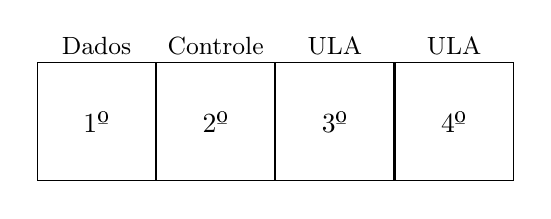
\begin{tikzpicture}
            \matrix[matrix of nodes, 
                    nodes in empty cells,
                    nodes={draw, minimum size=1.5cm, anchor=center},
                    column sep=0pt] (m) {
            {\text{1º}} & {\text{2º}} & {\text{3º}} & {\text{4º}} \\
            };

            \node[yshift=6pt] at (m-1-1.north) {\small Dados};
            \node[yshift=6pt] at (m-1-2.north) {\small Controle};
            \node[yshift=6pt] at (m-1-3.north) {\small ULA};
            \node[yshift=6pt] at (m-1-4.north) {\small ULA};
        \end{tikzpicture}
    \end{figure}

    \subsection{Motivações e Instruções}

    Para este processador gostariamos de dar a maior quantidade de operações lógicas possíveis ao programador e uma facilidade maior para mexer com loops, adicionando outra instrução branch de controle. Além disso, para que a utilização de predicados seja viável, adaptamos a ISA de modo que ela possua um conjunto de instruções específicas para cada uma das lanes do VLIW e instruções para settar o predicado na parte de controle

    %EXPLICAR AS 2 INSTRUÇÕES EXTRAS IMPLEMENTADAS

    \subsubsection{Multi Operations}


    \begin{table}[h]
      \captionsetup{labelformat=empty, skip=0pt}
      \caption{\textbf{Formato Novo:} Tipo Misto}
      \centering
      \rowcolors{1}{white}{red!20} 
      \begin{tabular}{|c|*{8}{c|}}
        \hline
        \rowcolor{red!50}
        \multicolumn{9}{|c|}{\textbf{Tipo INC}} \\ \hline
        \textbf{Bits} & 7 & 6 & 5 & 4 & 3 & 2 & 1 & 0 \\ \hline
        & \multicolumn{4}{c|}{\textbf{Opcode}} & \multicolumn{2}{c|}{\textbf{Ra}} & \multicolumn{2}{c|}{\textbf{Imm Unsigned}} \\ \hline
      \end{tabular}
    \end{table}

    % fazer tabela das suas operações

    \subsubsection{Move}

    \subsubsection{Predicação}

    %EXPLICAR SOBRE AS INSTRUÇÕES DE SET E AS INSTRUÇÕES QUE UTILIZARÃO PREDICAÇÃO EXPLICAR REGISTRADOR PR (PREDICADO)

    \begin{table}[H]
      \centering
      \captionsetup{labelformat=empty, skip=0pt}
      \caption{\textbf{Lane 1 Instruções: Dados}}
      \rowcolors{1}{white}{gray!20} 
      \begin{tabular}{|c|*{4}{c|}}
        \hline
        \rowcolor{gray!50}
        \multicolumn{1}{|c|}{\textbf{Opcode}} & \multicolumn{1}{|c|}{\textbf{Tipo}} & \multicolumn{1}{|c|}{\textbf{Mnemonic}} & \multicolumn{1}{|c|}{\textbf{Nome}}        & \multicolumn{1}{|c|}{\textbf{Operação}}                      \\ \hline
        \multicolumn{5}{|c|}{\textbf{Dados}} \\ \hline 
        \multicolumn{1}{|c|}{\textbf{0000}}   & \multicolumn{1}{c|}{\textbf{R}}     & \multicolumn{1}{c|}{\textbf{ld}}        & \multicolumn{1}{c|}{\textbf{Load}}         & \multicolumn{1}{c|}{\textbf{R[ra] = M[ R[rb] ] if PR}}       \\ \hline
        \multicolumn{1}{|c|}{\textbf{0001}}   & \multicolumn{1}{c|}{\textbf{R}}     & \multicolumn{1}{c|}{\textbf{st}}        & \multicolumn{1}{c|}{\textbf{Store}}        & \multicolumn{1}{c|}{\textbf{M[ R[rb] ] = R[ra] if PR}}       \\ \hline
        \multicolumn{1}{|c|}{\textbf{0010}}   & \multicolumn{1}{c|}{\textbf{I}}     & \multicolumn{1}{c|}{\textbf{movh}}      & \multicolumn{1}{c|}{\textbf{Move High}}    & \multicolumn{1}{c|}{\textbf{R[0] = {Imm, R[0](3:0)} if PR}}  \\ \hline
        \multicolumn{1}{|c|}{\textbf{0011}}   & \multicolumn{1}{c|}{\textbf{I}}     & \multicolumn{1}{c|}{\textbf{movl}}      & \multicolumn{1}{c|}{\textbf{Move Low}}     & \multicolumn{1}{c|}{\textbf{R[0] = {R[0](7:4), Imm} if PR}}  \\ \hline
        \multicolumn{1}{|c|}{\textbf{0100}}   & \multicolumn{1}{c|}{\textbf{R}}     & \multicolumn{1}{c|}{\textbf{f-ld}}      & \multicolumn{1}{c|}{\textbf{!Load}}        & \multicolumn{1}{c|}{\textbf{R[ra] = M[ R[rb] ] if !PR}}      \\ \hline
        \multicolumn{1}{|c|}{\textbf{0101}}   & \multicolumn{1}{c|}{\textbf{R}}     & \multicolumn{1}{c|}{\textbf{f-st}}      & \multicolumn{1}{c|}{\textbf{!Store}}       & \multicolumn{1}{c|}{\textbf{M[ R[rb] ] = R[ra] if !PR}}      \\ \hline
        \multicolumn{1}{|c|}{\textbf{0110}}   & \multicolumn{1}{c|}{\textbf{I}}     & \multicolumn{1}{c|}{\textbf{f-movh}}    & \multicolumn{1}{c|}{\textbf{!Move High}}   & \multicolumn{1}{c|}{\textbf{R[0] = {Imm, R[0](3:0)} if !PR}} \\ \hline
        \multicolumn{1}{|c|}{\textbf{0111}}   & \multicolumn{1}{c|}{\textbf{I}}     & \multicolumn{1}{c|}{\textbf{f-movl}}    & \multicolumn{1}{c|}{\textbf{!Move Low}}    & \multicolumn{1}{c|}{\textbf{R[0] = {R[0](7:4), Imm} if !PR}} \\ \hline
        \multicolumn{1}{|c|}{\textbf{1000}}   & \multicolumn{1}{c|}{\textbf{EMPTY}} & \multicolumn{1}{c|}{\textbf{EMPTY}}     & \multicolumn{1}{c|}{\textbf{EMPTY}}        & \multicolumn{1}{c|}{\textbf{EMPTY}}                          \\ \hline
        \multicolumn{1}{|c|}{\textbf{1001}}   & \multicolumn{1}{c|}{\textbf{EMPTY}} & \multicolumn{1}{c|}{\textbf{EMPTY}}     & \multicolumn{1}{c|}{\textbf{EMPTY}}        & \multicolumn{1}{c|}{\textbf{EMPTY}}                          \\ \hline
        \multicolumn{1}{|c|}{\textbf{1010}}   & \multicolumn{1}{c|}{\textbf{EMPTY}} & \multicolumn{1}{c|}{\textbf{EMPTY}}     & \multicolumn{1}{c|}{\textbf{EMPTY}}        & \multicolumn{1}{c|}{\textbf{EMPTY}}                          \\ \hline
        \multicolumn{1}{|c|}{\textbf{1011}}   & \multicolumn{1}{c|}{\textbf{EMPTY}} & \multicolumn{1}{c|}{\textbf{EMPTY}}     & \multicolumn{1}{c|}{\textbf{EMPTY}}        & \multicolumn{1}{c|}{\textbf{EMPTY}}                          \\ \hline
        \multicolumn{1}{|c|}{\textbf{1100}}   & \multicolumn{1}{c|}{\textbf{EMPTY}} & \multicolumn{1}{c|}{\textbf{EMPTY}}     & \multicolumn{1}{c|}{\textbf{EMPTY}}        & \multicolumn{1}{c|}{\textbf{EMPTY}}                          \\ \hline
        \multicolumn{1}{|c|}{\textbf{1101}}   & \multicolumn{1}{c|}{\textbf{EMPTY}} & \multicolumn{1}{c|}{\textbf{EMPTY}}     & \multicolumn{1}{c|}{\textbf{EMPTY}}        & \multicolumn{1}{c|}{\textbf{EMPTY}}                          \\ \hline
        \multicolumn{1}{|c|}{\textbf{1110}}   & \multicolumn{1}{c|}{\textbf{EMPTY}} & \multicolumn{1}{c|}{\textbf{EMPTY}}     & \multicolumn{1}{c|}{\textbf{EMPTY}}        & \multicolumn{1}{c|}{\textbf{EMPTY}}                          \\ \hline
        \multicolumn{5}{|c|}{\textbf{Free Slot}}                                                                                                                                                                                          \\ \hline 
        \multicolumn{1}{|c|}{\textbf{1111}}   & \multicolumn{1}{c|}{\textbf{R}}     & \multicolumn{1}{c|}{\textbf{nop}}       & \multicolumn{1}{c|}{\textbf{No Operation}} & \multicolumn{1}{c|}{\textbf{}}                               \\ \hline
      \end{tabular}
    \end{table}

    \begin{table}[H]
      \centering
      \captionsetup{labelformat=empty, skip=0pt}
      \caption{\textbf{Lane 2 Instruções: Controle}}
      \rowcolors{1}{white}{gray!20} 
      \noindent\hspace*{-2.5cm}
      \begin{tabular}{|c|*{4}{c|}}
        \hline
        \rowcolor{gray!50}
        \multicolumn{1}{|c|}{\textbf{Opcode}} & \multicolumn{1}{|c|}{\textbf{Tipo}} & \multicolumn{1}{|c|}{\textbf{Mnemonic}} & \multicolumn{1}{|c|}{\textbf{Nome}}                     & \multicolumn{1}{|c|}{\textbf{Operação}}                               \\ \hline
        \multicolumn{5}{|c|}{\textbf{Controle}} \\ \hline 
        \multicolumn{1}{|c|}{\textbf{0000}}   & \multicolumn{1}{c|}{\textbf{R}}     & \multicolumn{1}{c|}{\textbf{brzr}}      & \multicolumn{1}{c|}{\textbf{Branch On Zero Register}}   & \multicolumn{1}{c|}{\textbf{if (R[ra] == 0) PC = R[rb] if PR}}        \\ \hline
        \multicolumn{1}{|c|}{\textbf{0001}}   & \multicolumn{1}{c|}{\textbf{I}}     & \multicolumn{1}{c|}{\textbf{brzi}}      & \multicolumn{1}{c|}{\textbf{Branch On Zero Immediate}}  & \multicolumn{1}{c|}{\textbf{if (R[0] == 0) PC = PC + Imm if PR}}      \\ \hline
        \multicolumn{1}{|c|}{\textbf{0010}}   & \multicolumn{1}{c|}{\textbf{R}}     & \multicolumn{1}{c|}{\textbf{jr}}        & \multicolumn{1}{c|}{\textbf{Jump Register}}             & \multicolumn{1}{c|}{\textbf{PC = R[rb] if PR}}                        \\ \hline
        \multicolumn{1}{|c|}{\textbf{0011}}   & \multicolumn{1}{c|}{\textbf{R}}     & \multicolumn{1}{c|}{\textbf{mov}}       & \multicolumn{1}{c|}{\textbf{Move}}                      & \multicolumn{1}{c|}{\textbf{R[ra] = R[rb] if PR}}                     \\ \hline
        \multicolumn{1}{|c|}{\textbf{0100}}   & \multicolumn{1}{c|}{\textbf{R}}     & \multicolumn{1}{c|}{\textbf{f-brzr}}    & \multicolumn{1}{c|}{\textbf{!Branch On Zero Register}}  & \multicolumn{1}{c|}{\textbf{if (R[ra] == 0) PC = R[rb] if !PR}}       \\ \hline
        \multicolumn{1}{|c|}{\textbf{0101}}   & \multicolumn{1}{c|}{\textbf{I}}     & \multicolumn{1}{c|}{\textbf{f-brzi}}    & \multicolumn{1}{c|}{\textbf{!Branch On Zero Immediate}} & \multicolumn{1}{c|}{\textbf{if (R[0] == 0) PC = PC + Imm if !PR}}     \\ \hline
        \multicolumn{1}{|c|}{\textbf{0110}}   & \multicolumn{1}{c|}{\textbf{R}}     & \multicolumn{1}{c|}{\textbf{f-jr}}      & \multicolumn{1}{c|}{\textbf{!Jump Register}}            & \multicolumn{1}{c|}{\textbf{PC = R[rb] if !PR}}                       \\ \hline
        \multicolumn{1}{|c|}{\textbf{0111}}   & \multicolumn{1}{c|}{\textbf{R}}     & \multicolumn{1}{c|}{\textbf{f-mov}}     & \multicolumn{1}{c|}{\textbf{!Move}}                     & \multicolumn{1}{c|}{\textbf{R[ra] = R[rb] if !PR}}                    \\ \hline
        \multicolumn{5}{|c|}{\textbf{Setters}}                                                                                                                                                                                                                  \\ \hline 
        \multicolumn{1}{|c|}{\textbf{1000}}   & \multicolumn{1}{c|}{\textbf{R}}     & \multicolumn{1}{c|}{\textbf{sgt}}       & \multicolumn{1}{c|}{\textbf{Set Greater Than}}          & \multicolumn{1}{c|}{\textbf{if R[ra] > R[rb] R[pr] := 1; R[pr] := 0}} \\ \hline
        \multicolumn{1}{|c|}{\textbf{1001}}   & \multicolumn{1}{c|}{\textbf{R}}     & \multicolumn{1}{c|}{\textbf{slt}}       & \multicolumn{1}{c|}{\textbf{Set Less Than}}             & \multicolumn{1}{c|}{\textbf{if R[ra] < R[rb] R[pr] := 1; R[pr] := 0}} \\ \hline
        \multicolumn{1}{|c|}{\textbf{1010}}   & \multicolumn{1}{c|}{\textbf{R}}     & \multicolumn{1}{c|}{\textbf{seq}}       & \multicolumn{1}{c|}{\textbf{Set Equal}}                 & \multicolumn{1}{c|}{\textbf{if R[ra] = R[rb] R[pr] := 1; R[pr] := 0}} \\ \hline
        \multicolumn{1}{|c|}{\textbf{1011}}   & \multicolumn{1}{c|}{\textbf{R}}     & \multicolumn{1}{c|}{\textbf{strue}}     & \multicolumn{1}{c|}{\textbf{Set True}}                  & \multicolumn{1}{c|}{\textbf{R[pr] := 1}}                              \\ \hline
        \multicolumn{1}{|c|}{\textbf{1100}}   & \multicolumn{1}{c|}{\textbf{EMPTY}} & \multicolumn{1}{c|}{\textbf{EMPTY}}     & \multicolumn{1}{c|}{\textbf{EMPTY}}                     & \multicolumn{1}{c|}{\textbf{EMPTY}}                                   \\ \hline
        \multicolumn{1}{|c|}{\textbf{1101}}   & \multicolumn{1}{c|}{\textbf{EMPTY}} & \multicolumn{1}{c|}{\textbf{EMPTY}}     & \multicolumn{1}{c|}{\textbf{EMPTY}}                     & \multicolumn{1}{c|}{\textbf{EMPTY}}                                   \\ \hline
        \multicolumn{1}{|c|}{\textbf{1110}}   & \multicolumn{1}{c|}{\textbf{EMPTY}} & \multicolumn{1}{c|}{\textbf{EMPTY}}     & \multicolumn{1}{c|}{\textbf{EMPTY}}                     & \multicolumn{1}{c|}{\textbf{EMPTY}}                                   \\ \hline
        \multicolumn{5}{|c|}{\textbf{Free Slot}}                                                                                                                                                                                                                \\ \hline 
        \multicolumn{1}{|c|}{\textbf{1111}}   & \multicolumn{1}{c|}{\textbf{R}}     & \multicolumn{1}{c|}{\textbf{nop}}       & \multicolumn{1}{c|}{\textbf{No Operation}}              & \multicolumn{1}{c|}{\textbf{}}                                        \\ \hline
      \end{tabular}
    \end{table}

    \begin{table}[H]
      \centering
      \captionsetup{labelformat=empty, skip=0pt}
      \caption{\textbf{Lanes 3 e 4 Instruções: Aritmética e Lógica}}
      \rowcolors{1}{white}{gray!20} 
      \noindent\hspace*{-1cm}%
      \begin{tabular}{|c|*{4}{c|}}
        \hline
        \rowcolor{gray!50}
        \multicolumn{1}{|c|}{\textbf{Opcode}} & \multicolumn{1}{|c|}{\textbf{Tipo}} & \multicolumn{1}{|c|}{\textbf{Mnemonic}} & \multicolumn{1}{|c|}{\textbf{Nome}}                & \multicolumn{1}{|c|}{\textbf{Operação}}                            \\ \hline
        \multicolumn{5}{|c|}{\textbf{Aritmética e Lógica}} \\ \hline 
        \multicolumn{1}{|c|}{\textbf{0000}}   & \multicolumn{1}{c|}{\textbf{R}}     & \multicolumn{1}{c|}{\textbf{add}}       & \multicolumn{1}{c|}{\textbf{Add}}                  & \multicolumn{1}{c|}{\textbf{R[ra] = R[ra] + R[rb] if PR}}          \\ \hline
        \multicolumn{1}{|c|}{\textbf{0001}}   & \multicolumn{1}{c|}{\textbf{R}}     & \multicolumn{1}{c|}{\textbf{sub}}       & \multicolumn{1}{c|}{\textbf{Sub}}                  & \multicolumn{1}{c|}{\textbf{R[ra] = R[ra] - R[rb] if PR}}          \\ \hline
        \multicolumn{1}{|c|}{\textbf{0010}}   & \multicolumn{1}{c|}{\textbf{M}}     & \multicolumn{1}{c|}{\textbf{mult-op}}   & \multicolumn{1}{c|}{\textbf{Multi Operations}}     & \multicolumn{1}{c|}{\textbf{R[ra] = R[ra] OP R[0] | !R[0] if PR}}  \\ \hline
        \multicolumn{1}{|c|}{\textbf{0011}}   & \multicolumn{1}{c|}{\textbf{R}}     & \multicolumn{1}{c|}{\textbf{or}}        & \multicolumn{1}{c|}{\textbf{Or}}                   & \multicolumn{1}{c|}{\textbf{R[ra] = R[ra] | R[rb] if PR}}          \\ \hline
        \multicolumn{1}{|c|}{\textbf{0100}}   & \multicolumn{1}{c|}{\textbf{R}}     & \multicolumn{1}{c|}{\textbf{not}}       & \multicolumn{1}{c|}{\textbf{Not}}                  & \multicolumn{1}{c|}{\textbf{R[ra] = ! R[rb] if PR}}                \\ \hline
        \multicolumn{1}{|c|}{\textbf{0101}}   & \multicolumn{1}{c|}{\textbf{R}}     & \multicolumn{1}{c|}{\textbf{slr}}       & \multicolumn{1}{c|}{\textbf{Shift Left Register}}  & \multicolumn{1}{c|}{\textbf{R[ra] = R[ra] << R[rb] if PR}}         \\ \hline
        \multicolumn{1}{|c|}{\textbf{0110}}   & \multicolumn{1}{c|}{\textbf{R}}     & \multicolumn{1}{c|}{\textbf{srr}}       & \multicolumn{1}{c|}{\textbf{Shift Right Register}} & \multicolumn{1}{c|}{\textbf{R[ra] = R[ra] >> R[rb] if PR}}         \\ \hline
        \multicolumn{1}{|c|}{\textbf{0111}}   & \multicolumn{1}{c|}{\textbf{EMPTY}} & \multicolumn{1}{c|}{\textbf{EMPTY}}     & \multicolumn{1}{c|}{\textbf{EMPTY}}                & \multicolumn{1}{c|}{\textbf{EMPTY}}                                \\ \hline
        \multicolumn{1}{|c|}{\textbf{1000}}   & \multicolumn{1}{c|}{\textbf{R}}     & \multicolumn{1}{c|}{\textbf{f-add}}     & \multicolumn{1}{c|}{\textbf{Add}}                  & \multicolumn{1}{c|}{\textbf{R[ra] = R[ra] + R[rb] if !PR}}         \\ \hline
        \multicolumn{1}{|c|}{\textbf{1001}}   & \multicolumn{1}{c|}{\textbf{R}}     & \multicolumn{1}{c|}{\textbf{f-sub}}     & \multicolumn{1}{c|}{\textbf{Sub}}                  & \multicolumn{1}{c|}{\textbf{R[ra] = R[ra] - R[rb] if !PR}}         \\ \hline
        \multicolumn{1}{|c|}{\textbf{1010}}   & \multicolumn{1}{c|}{\textbf{M}}     & \multicolumn{1}{c|}{\textbf{f-mult-op}} & \multicolumn{1}{c|}{\textbf{Multi Operations}}     & \multicolumn{1}{c|}{\textbf{R[ra] = R[ra] OP R[0] | !R[0] if !PR}} \\ \hline
        \multicolumn{1}{|c|}{\textbf{1011}}   & \multicolumn{1}{c|}{\textbf{R}}     & \multicolumn{1}{c|}{\textbf{f-or}}      & \multicolumn{1}{c|}{\textbf{Or}}                   & \multicolumn{1}{c|}{\textbf{R[ra] = R[ra] | R[rb] if !PR}}         \\ \hline
        \multicolumn{1}{|c|}{\textbf{1100}}   & \multicolumn{1}{c|}{\textbf{R}}     & \multicolumn{1}{c|}{\textbf{f-not}}     & \multicolumn{1}{c|}{\textbf{Not}}                  & \multicolumn{1}{c|}{\textbf{R[ra] = ! R[rb] if !PR}}               \\ \hline
        \multicolumn{1}{|c|}{\textbf{1101}}   & \multicolumn{1}{c|}{\textbf{R}}     & \multicolumn{1}{c|}{\textbf{f-slr}}     & \multicolumn{1}{c|}{\textbf{Shift Left Register}}  & \multicolumn{1}{c|}{\textbf{R[ra] = R[ra] << R[rb] if !PR}}        \\ \hline
        \multicolumn{1}{|c|}{\textbf{1110}}   & \multicolumn{1}{c|}{\textbf{R}}     & \multicolumn{1}{c|}{\textbf{f-srr}}     & \multicolumn{1}{c|}{\textbf{Shift Right Register}} & \multicolumn{1}{c|}{\textbf{R[ra] = R[ra] >> R[rb] if !PR}}        \\ \hline
        \multicolumn{5}{|c|}{\textbf{Free Slot}}                                                                                                                                                                                                        \\ \hline 
        \multicolumn{1}{|c|}{\textbf{1111}}   & \multicolumn{1}{c|}{\textbf{R}}     & \multicolumn{1}{c|}{\textbf{nop}}       & \multicolumn{1}{c|}{\textbf{No Operation}}         & \multicolumn{1}{c|}{\textbf{}}                                     \\ \hline
      \end{tabular}
    \end{table}

    % CONCERTAR UTF 8 NAS TABELAS


    \section{Implementação e Organização}

    % EXPLICAR DETALHES DA IMPLEMENTAÇÃO DO HARDWARE, COLOCAR TABELAS DE CONTROLE, DIAGRAMA DE CAIXAS E ETC


    \begin{table}[H]
      \captionsetup{labelformat=empty, skip=0pt}
      \caption{\textbf{Lane 1 Controle: Dados}}
      \centering
      \resizebox{\textwidth}{!}{
        \begin{tabular}{@{} l c c c c c c @{}}
          \toprule
          Mnemonic & OPCODE & MOVL & MOVH & ST & LD & TRUE  \\
          \midrule
          ld       & 0000   & 0    & 0    & 0  & 1  & 1     \\
          st       & 0001   & 0    & 0    & 1  & 0  & 1     \\
          movh     & 0010   & 0    & 1    & 0  & 0  & 1     \\
          movl     & 0011   & 1    & 0    & 0  & 0  & 1     \\
          f-ld     & 0100   & 0    & 0    & 0  & 1  & 0     \\
          f-st     & 0101   & 0    & 0    & 1  & 0  & 0     \\
          f-movh   & 0110   & 0    & 1    & 0  & 0  & 0     \\
          f-movl   & 0111   & 1    & 0    & 0  & 0  & 0     \\
          empty    & 1000   & x    & x    & x  & x  & x     \\
          empty    & 1001   & x    & x    & x  & x  & x     \\
          empty    & 1010   & x    & x    & x  & x  & x     \\
          empty    & 1011   & x    & x    & x  & x  & x     \\
          empty    & 1100   & x    & x    & x  & x  & x     \\
          empty    & 1101   & x    & x    & x  & x  & x     \\
          empty    & 1110   & x    & x    & x  & x  & x     \\
          nop      & 1111   & 0    & 0    & 0  & 0  & x     \\
          \bottomrule
        \end{tabular}
      }
    \end{table}

    \begin{table}[H]
      \captionsetup{labelformat=empty, skip=0pt}
      \caption{\textbf{Lane 2 Controle: Branches}}
      \centering
      \resizebox{\textwidth}{!}{
        \begin{tabular}{@{} l c c c c c c c c @{}}
          \toprule
          Mnemonic & OPCODE & BOZR & JR & BOZI & MOVE & TRUE & PR\_OP & W\_PR  \\
          \midrule
          brzr     & 0000   & 1    & 0  & 0    & 0    & 1    & xx    & 0     \\
          brzi     & 0001   & 0    & 0  & 1    & 0    & 1    & xx    & 0     \\
          jr       & 0010   & 0    & 1  & 0    & 0    & 1    & xx    & 0     \\
          mov      & 0011   & 0    & 0  & 0    & 1    & 1    & xx    & 0     \\
          f-brzr   & 0100   & 1    & 0  & 0    & 0    & 0    & xx    & 0     \\
          f-brzi   & 0101   & 0    & 0  & 1    & 0    & 0    & xx    & 0     \\
          f-jr     & 0110   & 0    & 1  & 0    & 0    & 0    & xx    & 0     \\
          f-mov    & 0111   & 0    & 0  & 0    & 1    & 0    & xx    & 0     \\
          sgt      & 1000   & 0    & 0  & 0    & 0    & x    & 00    & 1     \\
          slt      & 1001   & 0    & 0  & 0    & 0    & x    & 10    & 1     \\
          seq      & 1010   & 0    & 0  & 0    & 0    & x    & 01    & 1     \\
          strue    & 1011   & 0    & 0  & 0    & 0    & x    & 11    & 1     \\
          empty    & 1100   & x    & x  & x    & x    & x    & xx    & x     \\
          empty    & 1101   & x    & x  & x    & x    & x    & xx    & x     \\
          empty    & 1110   & x    & x  & x    & x    & x    & xx    & x     \\
          nop      & 1111   & 0    & 0  & 0    & 0    & x    & xx    & 0     \\
          \bottomrule
        \end{tabular}
      }
    \end{table}

    \begin{table}[H]
      \captionsetup{labelformat=empty, skip=0pt}
      \caption{\textbf{Lane 3 e 4 Controle: Aritmética e Lógica}}
      \centering
      \resizebox{\textwidth}{!}{
        \begin{tabular}{@{} l c c c c @{}}
          \toprule
          Mnemonic & OPCODE & OP\_ULA & WE & TRUE  \\
          \midrule
          add       & 0000   & 000    & 1  & 1     \\
          sub       & 0001   & 001    & 1  & 1     \\
          mult-op   & 0010   & 010    & 1  & 1     \\
          or        & 0011   & 011    & 1  & 1     \\
          not       & 0100   & 100    & 1  & 1     \\
          slr       & 0101   & 101    & 1  & 1     \\
          srr       & 0110   & 110    & 1  & 1     \\
          empty     & 0111   & xxx    & x  & x     \\
          f-add     & 1000   & 000    & 1  & 0     \\
          f-sub     & 1001   & 001    & 1  & 0     \\
          f-mult-op & 1010   & 010    & 1  & 0     \\
          f-or      & 1011   & 011    & 1  & 0     \\
          f-not     & 1100   & 100    & 1  & 0     \\
          f-slr     & 1101   & 101    & 1  & 0     \\
          f-srr     & 1110   & 110    & 1  & 0     \\
          nop       & 1111   & 111    & 0  & x     \\
          \bottomrule
        \end{tabular}
      }
    \end{table}



    \subsubsection{Instrução 1}

    \subsubsection{Instrução 2}

    \subsubsection{Predicação}

    % EXPLICAR COMO FOI IMPLEMENTADO
    % TABELO DO PR_OP


    \section{Resultado}

    % FINALIZAR MOSTRANDO O ASSEMBLY E CONCLUSÃO

\end{document} 
